\chapter{Database MySQL}

\section{Pengenalan Database MySQL}

\subsection{Pendahuluan}

MySQL adalah salah satu sistem manajemen basis data relasional (RDBMS) yang paling populer di dunia. MySQL digunakan secara luas karena kecepatan, skalabilitas, dan kemudahan penggunaannya. Dalam pengembangan aplikasi Java, MySQL sering digunakan sebagai database untuk menyimpan dan mengelola data. Untuk menghubungkan aplikasi Java dengan MySQL, kita menggunakan Java Database Connectivity (JDBC).

\subsection{Langkah-langkah Menggunakan MySQL di Java}

Berikut adalah langkah-langkah untuk menghubungkan aplikasi Java dengan database MySQL:

\subsubsection{1. Instalasi MySQL}

Sebelum memulai, pastikan Anda telah menginstal MySQL di sistem Anda. Anda dapat mengunduh dan menginstalnya dari situs web resmi MySQL.\\

Silahkan tonton video berikut untuk panduan lebih lanjut\\ \url{https://www.youtube.com/watch?v=Ev_h-6OkvA4&list=PLl9D0-J08TNXNjQPwWMVOUrqA-oiDrGyk&index=13}

\subsubsection{2. Menyiapkan Database MySQL}

Setelah MySQL terinstal, Anda dapat membuat database yang akan digunakan dalam aplikasi Java Anda. Misalnya, kita akan membuat database \texttt{studentdb} dan tabel \texttt{students} untuk menyimpan data mahasiswa. 

Untuk bagian ini, kamu dapat membuat database dengan alternatif seperti PHPMyAdmin, DBeaver, atau MySQL Workbench(Hanya untul SQL versi 8.5 kebawah). Bahkan kamu juga bisa membuat tabel dengan command prompt saja (lihat pada link youtube untuk tata cara dengan MySQL Workbench)

\subsubsection{2.1 Persiapan Database dengan MySQL dan DBeaver}

Sebelum memasuki persiapan ini, pastikan telah menonton video untuk mengetahui cara mengaktifkan koneksi dengan CLI (Command Line).

\begin{itemize}
	\item Download Dbeaver melalui link berikut \\ \url{https://dbeaver.io/download/}
	
	\item Setelah instalasi telah dilakukan, buka Dbeaver
	
	\item Pada bagian kiri atas, pilih New Database Connection
	
	\item Pilih MySQL , kemudian klik Next\\
	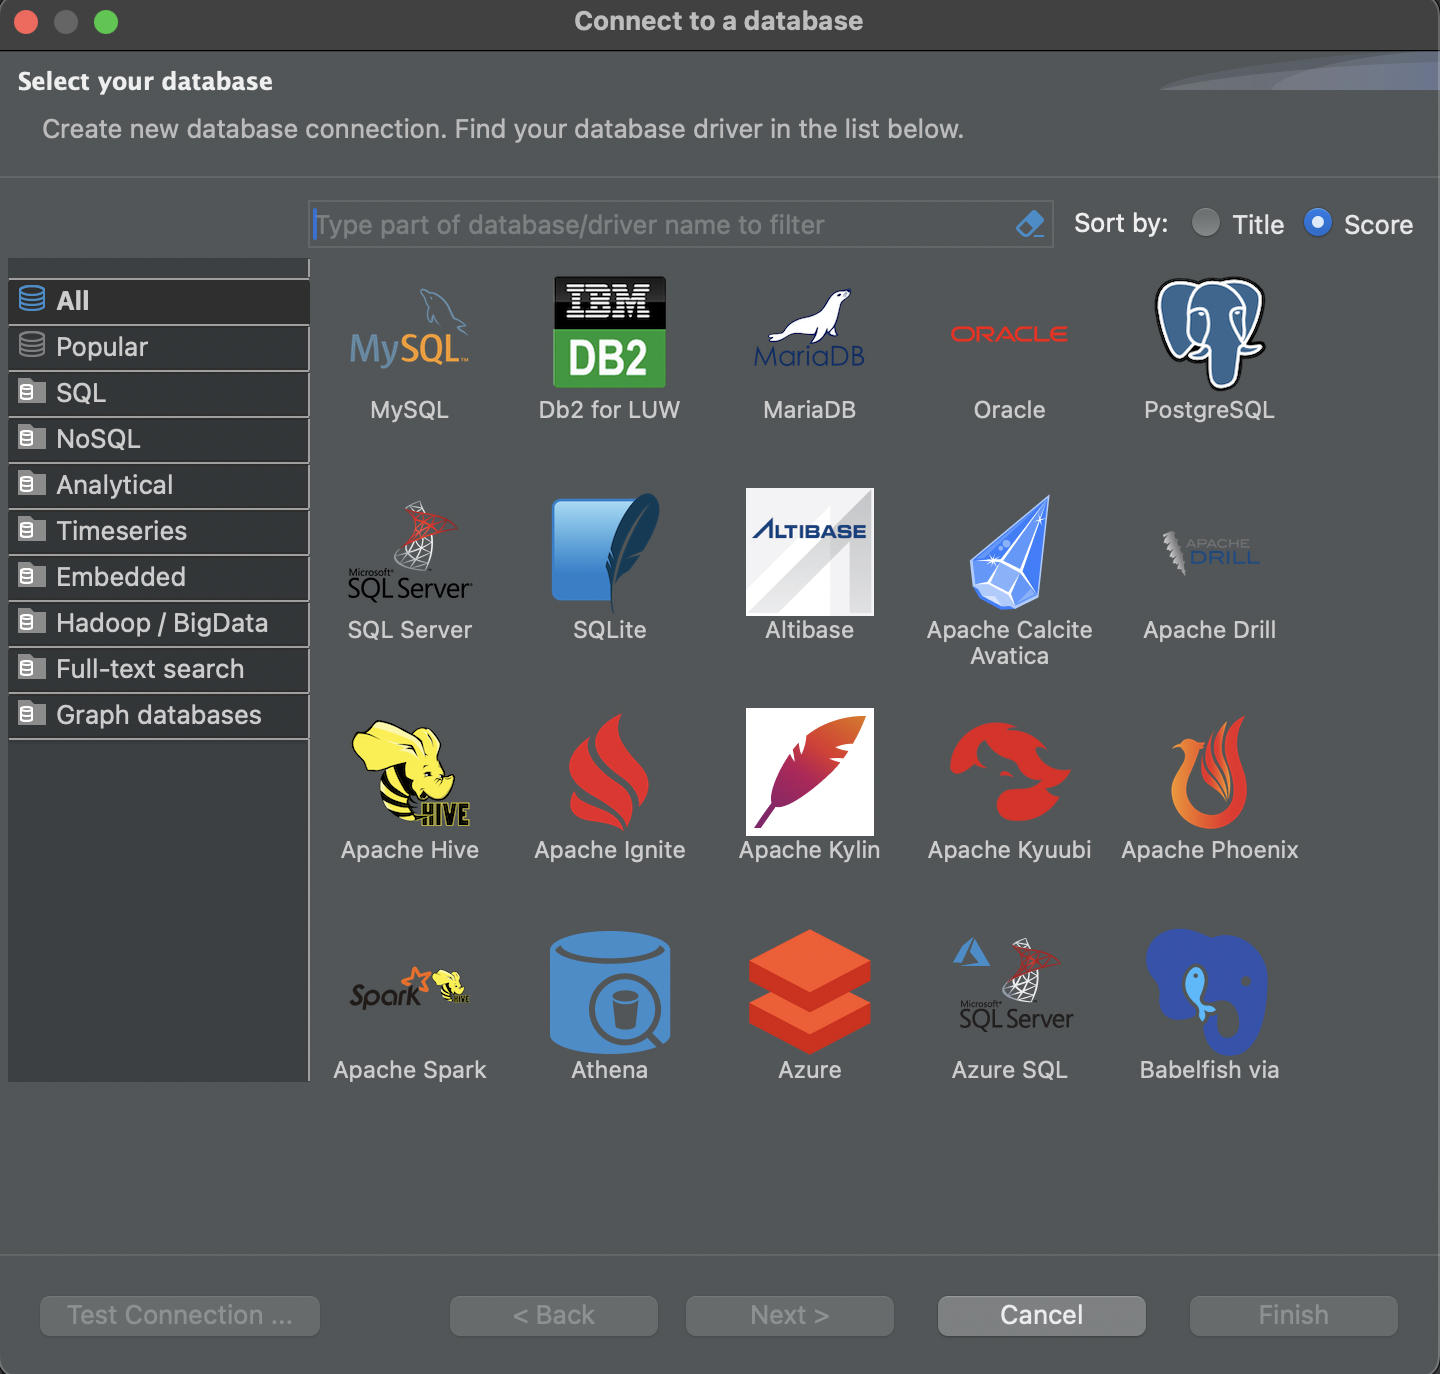
\includegraphics[width=0.33\textwidth]{assets/pertemuan12/dbeaver-select-connection.png}
	
	\item Pada halaman Connection Settings, tidak perlu mengubah konten yang ada, langsung klik Finish\\
	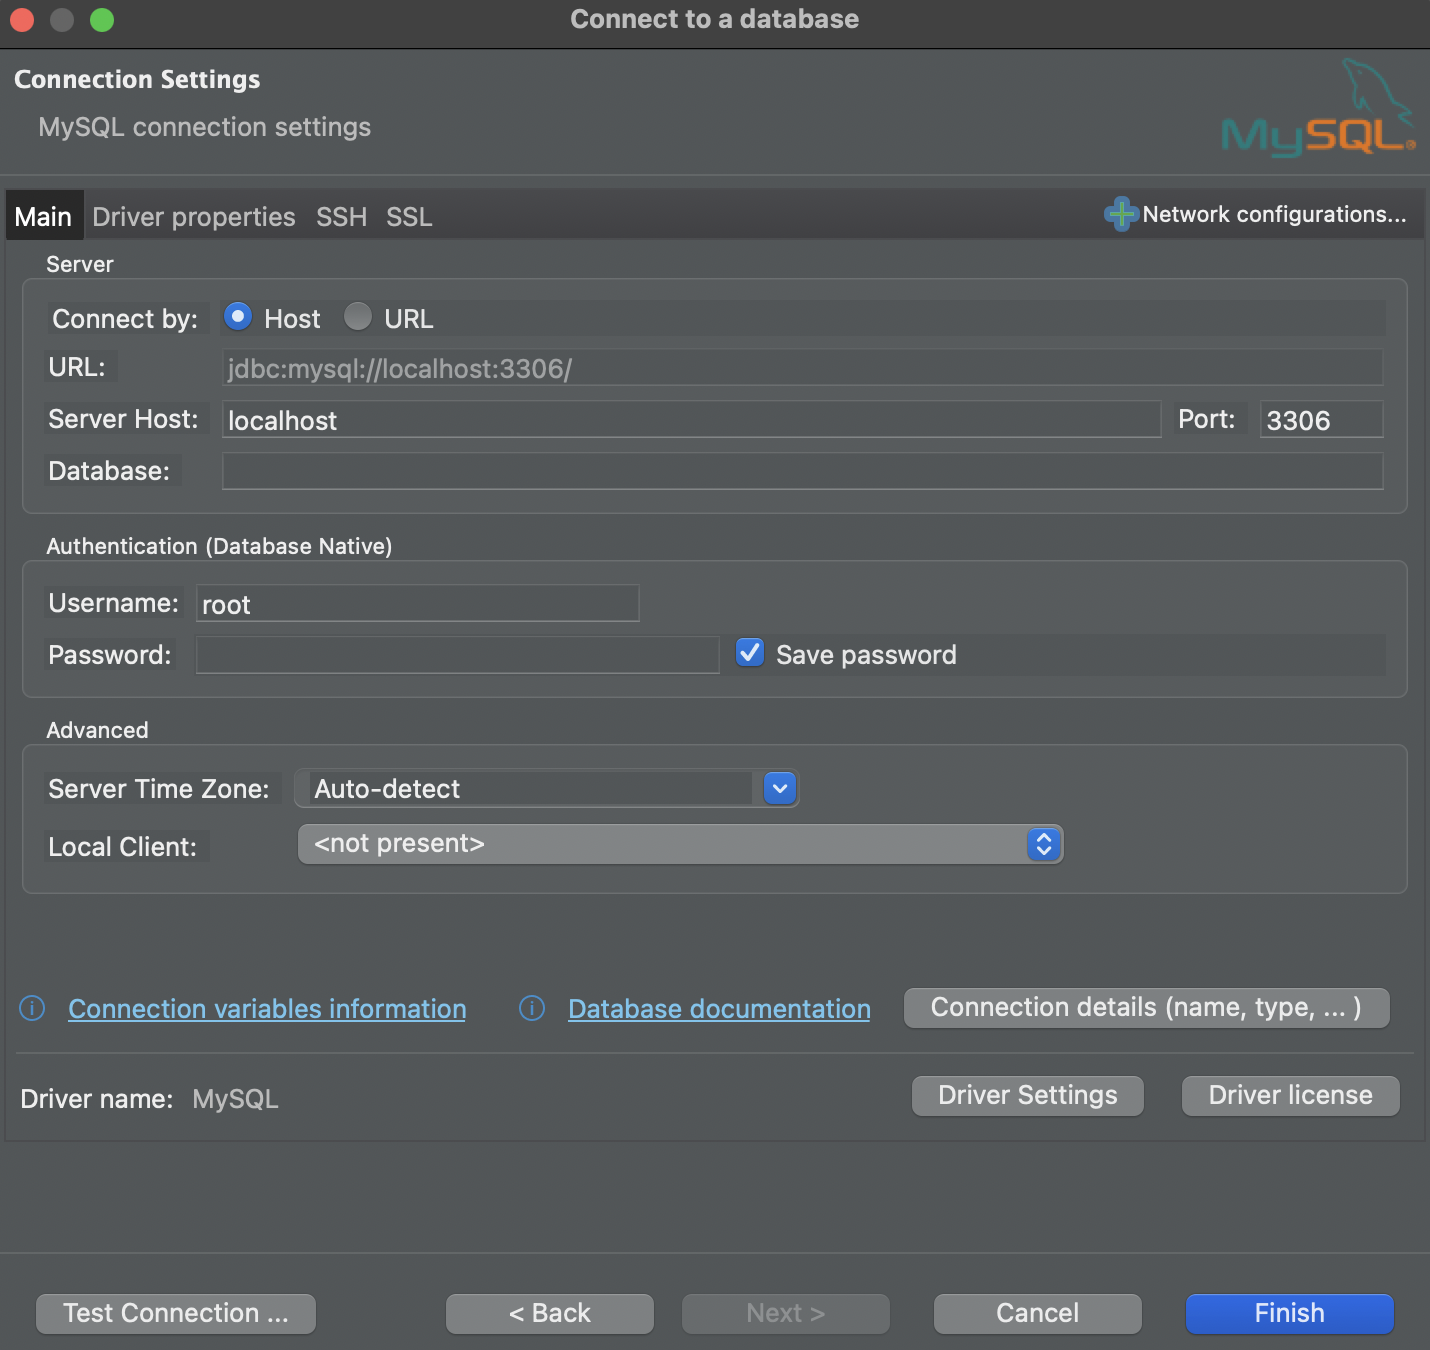
\includegraphics[width=0.33\textwidth]{assets/pertemuan12/dbeaver-connection-settings.png}
	
	\item Setelah telah terkoneksi, expand bagian koneksi yang telah dibuat 
	
	\item Expand menu Databases
	
	\item Klik kanan pada menu Databases, kemudian pilih Create New Databases
	
	\item Masukkan nama studentdb pada nama database, kemudian klik OK
	
	\item Pada nama database studentdb, klik kanan, pilih SQL Editor dan pilih create New Script
	
	\item Masukkan script berikut, kemudian run
	\begin{lstlisting}[style=JavaStyle]
		USE studentdb;
		
		CREATE TABLE students (
			id INT AUTO_INCREMENT PRIMARY KEY,
			name VARCHAR(50),
			age INT,
			major VARCHAR(50)
		);
	\end{lstlisting}
	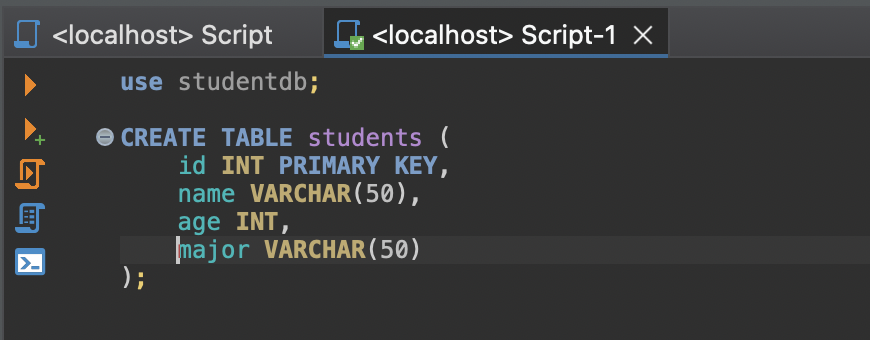
\includegraphics[width=0.33\textwidth]{assets/pertemuan12/dbeaver-script-create-table.png}
	
	\item Database dan table sudah berhasil dibuat!\\
	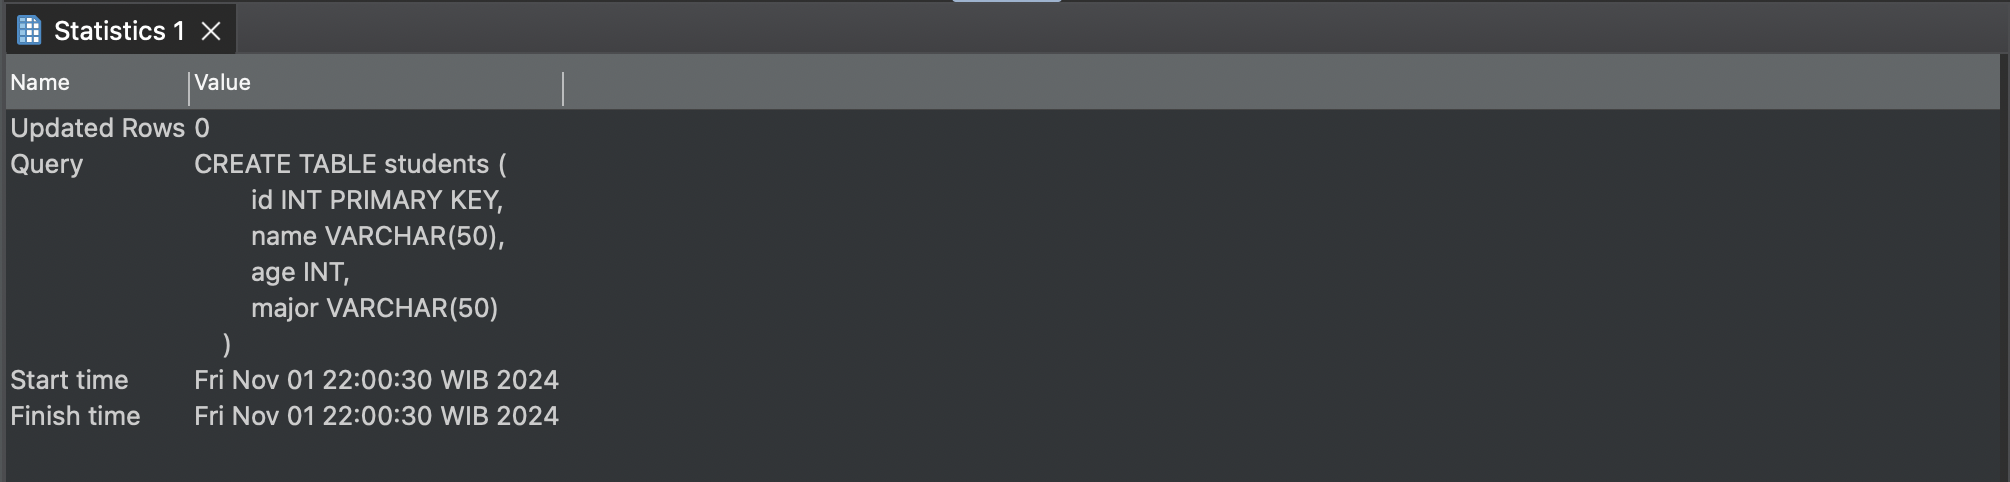
\includegraphics[width=0.8\textwidth]{assets/pertemuan12/dbeaver-table-success-script.png}
	
\end{itemize}


\section{Create Database}

Untuk memulai proyek dalam MySQL, pertama-tama kita perlu membuat database. Database adalah kumpulan tabel yang akan menyimpan data yang diperlukan dalam suatu aplikasi. Berikut adalah dua contoh perintah untuk membuat database beserta cara membuktikan keberhasilannya.

\subsection*{Contoh 1: Membuat Database Sederhana}
Kode berikut membuat database bernama \texttt{sekolah}.

\begin{lstlisting}[style=sql]
CREATE DATABASE sekolah;
\end{lstlisting}

Untuk memastikan database telah dibuat, kita bisa menggunakan perintah \texttt{SHOW DATABASES;} yang akan menampilkan daftar seluruh database yang ada di MySQL. Jika nama database yang kita buat muncul dalam daftar, maka pembuatan database telah berhasil.

\begin{lstlisting}[style=sql]
SHOW DATABASES;
\end{lstlisting}

Jika \texttt{sekolah} muncul dalam hasil perintah \texttt{SHOW DATABASES;}, maka database berhasil dibuat.

\subsection*{Contoh 2: Membuat Database dengan Karakteristik Khusus}
Pada contoh ini, kita membuat database bernama \texttt{perpustakaan} dengan karakter set \texttt{utf8mb4} dan collation \texttt{utf8mb4\_unicode\_ci}.

\begin{lstlisting}[style=sql]
CREATE DATABASE perpustakaan
CHARACTER SET utf8mb4
COLLATE utf8mb4_unicode_ci;
\end{lstlisting}

Untuk membuktikan bahwa database \texttt{perpustakaan} berhasil dibuat dengan karakteristik tersebut, kita dapat menjalankan \texttt{SHOW CREATE DATABASE perpustakaan;} untuk melihat detailnya.

\begin{lstlisting}[style=sql]
SHOW CREATE DATABASE perpustakaan;
\end{lstlisting}

Jika output menunjukkan \texttt{utf8mb4} dan \texttt{utf8mb4\_unicode\_ci} pada konfigurasi database \texttt{perpustakaan}, maka database berhasil dibuat sesuai karakteristik yang diinginkan.

\section{Create Table}

Setelah membuat database, langkah selanjutnya adalah membuat tabel untuk menyimpan data. Tabel terdiri dari kolom-kolom yang masing-masing mendefinisikan tipe data yang dapat disimpan.

\subsection*{Contoh 1: Membuat Tabel Siswa}
Contoh berikut membuat tabel bernama \texttt{siswa} yang menyimpan informasi tentang siswa seperti \texttt{id}, \texttt{nama}, dan \texttt{umur}.

\begin{lstlisting}[style=sql]
CREATE TABLE siswa (
id INT PRIMARY KEY,
nama VARCHAR(50),
umur INT
);
\end{lstlisting}

Untuk memastikan tabel \texttt{siswa} berhasil dibuat, pilih database \texttt{sekolah} terlebih dahulu, lalu gunakan perintah \texttt{SHOW TABLES;}.

\begin{lstlisting}[style=sql]
USE sekolah;
SHOW TABLES;
\end{lstlisting}

Jika tabel \texttt{siswa} muncul dalam hasil perintah \texttt{SHOW TABLES;}, maka tabel telah berhasil dibuat.

Selanjutnya, kita dapat menggunakan perintah \texttt{DESCRIBE} untuk melihat struktur tabel dan memastikan kolom serta tipe datanya sesuai.

\begin{lstlisting}[style=sql]
DESCRIBE siswa;
\end{lstlisting}

Output dari perintah ini akan menampilkan kolom \texttt{id}, \texttt{nama}, dan \texttt{umur} beserta tipe data masing-masing. Jika output sesuai dengan struktur yang direncanakan, maka pembuatan tabel \texttt{siswa} berhasil.

\subsection*{Contoh 2: Membuat Tabel Buku}
Berikut adalah contoh tabel \texttt{buku} yang menyimpan informasi tentang buku di perpustakaan dengan kolom \texttt{id\_buku}, \texttt{judul}, dan \texttt{penulis}.

\begin{lstlisting}[style=sql]
CREATE TABLE buku (
id_buku INT PRIMARY KEY,
judul VARCHAR(100),
penulis VARCHAR(50)
);
\end{lstlisting}

Untuk memastikan tabel \texttt{buku} berhasil dibuat, gunakan perintah \texttt{SHOW TABLES;} setelah memilih database yang tepat.

\begin{lstlisting}[style=sql]
USE sekolah;
SHOW TABLES;
\end{lstlisting}

Jika tabel \texttt{buku} muncul dalam hasil perintah \texttt{SHOW TABLES;}, maka pembuatan tabel berhasil.

Kita juga bisa menjalankan \texttt{DESCRIBE} untuk melihat detail kolom tabel \texttt{buku}.

\begin{lstlisting}[style=sql]
DESCRIBE buku;
\end{lstlisting}

Output dari perintah ini akan menampilkan kolom \texttt{id\_buku}, \texttt{judul}, dan \texttt{penulis} beserta tipe data masing-masing. Jika output sesuai dengan struktur yang direncanakan, maka tabel \texttt{buku} telah berhasil dibuat.

\section{Insert}

Perintah \texttt{INSERT} digunakan untuk menambahkan data ke dalam tabel. Berikut adalah dua contoh perintah \texttt{INSERT} beserta cara membuktikan keberhasilannya.

\subsection*{Contoh 1: Menambahkan Data ke Tabel Siswa}
Kode berikut menambahkan data ke tabel \texttt{siswa} yang telah dibuat sebelumnya.

\begin{lstlisting}[style=sql]
	INSERT INTO siswa (id, nama, umur)
	VALUES (1, 'Budi', 20);
\end{lstlisting}

Untuk memastikan bahwa data berhasil dimasukkan, kita dapat menggunakan perintah \texttt{SELECT} untuk menampilkan isi tabel \texttt{siswa}.

\begin{lstlisting}[style=sql]
	SELECT * FROM siswa;
\end{lstlisting}

Jika hasil perintah \texttt{SELECT} menampilkan data dengan \texttt{id = 1}, \texttt{nama = 'Budi'}, dan \texttt{umur = 20}, maka data berhasil ditambahkan.

\subsection*{Contoh 2: Menambahkan Data Lain ke Tabel Siswa}
Contoh berikut menambahkan data lain ke tabel \texttt{siswa}.

\begin{lstlisting}[style=sql]
	INSERT INTO siswa (id, nama, umur)
	VALUES (2, 'Siti', 22);
\end{lstlisting}

Untuk membuktikan bahwa data telah ditambahkan, gunakan perintah \texttt{SELECT} seperti sebelumnya:

\begin{lstlisting}[style=sql]
	SELECT * FROM siswa;
\end{lstlisting}

Jika data dengan \texttt{id = 2}, \texttt{nama = 'Siti'}, dan \texttt{umur = 22} muncul dalam hasil \texttt{SELECT}, maka perintah \texttt{INSERT} berhasil.

\section{Select}

Perintah \texttt{SELECT} digunakan untuk mengambil data dari tabel. Berikut adalah dua contoh penggunaan \texttt{SELECT} beserta cara memverifikasi hasilnya.

\subsection*{Contoh 1: Mengambil Semua Data dari Tabel Siswa}
Perintah berikut menampilkan semua data dari tabel \texttt{siswa}.

\begin{lstlisting}[style=sql]
	SELECT * FROM siswa;
\end{lstlisting}

Perintah ini akan menampilkan seluruh data dalam tabel \texttt{siswa}, termasuk data yang telah kita masukkan di bagian sebelumnya. Jika output menampilkan data sesuai yang diinput, maka perintah \texttt{SELECT} bekerja dengan benar.

\subsection*{Contoh 2: Mengambil Data Berdasarkan Kondisi}
Kode berikut mengambil data dari tabel \texttt{siswa} dengan kondisi tertentu, yaitu hanya siswa yang berumur lebih dari 20 tahun.

\begin{lstlisting}[style=sql]
	SELECT * FROM siswa
	WHERE umur > 20;
\end{lstlisting}

Jika output menampilkan data dengan \texttt{umur} lebih dari 20, maka perintah \texttt{SELECT} dengan kondisi \texttt{WHERE} berhasil. Sebagai contoh, data untuk \texttt{Siti} (umur 22) akan muncul dalam hasil, sedangkan \texttt{Budi} (umur 20) tidak akan muncul.

\section{Update}

Perintah \texttt{UPDATE} digunakan untuk memperbarui data dalam tabel. Berikut adalah dua contoh perintah \texttt{UPDATE} beserta cara membuktikan keberhasilannya.

\subsection*{Contoh 1: Memperbarui Umur Siswa}
Kode berikut memperbarui data umur siswa bernama \texttt{Budi} di tabel \texttt{siswa}.

\begin{lstlisting}[style=sql]
	UPDATE siswa
	SET umur = 21
	WHERE nama = 'Budi';
\end{lstlisting}

Untuk memastikan data berhasil diperbarui, kita dapat menggunakan perintah \texttt{SELECT} untuk melihat perubahan pada tabel \texttt{siswa}.

\begin{lstlisting}[style=sql]
	SELECT * FROM siswa
	WHERE nama = 'Budi';
\end{lstlisting}

Jika hasil menunjukkan bahwa \texttt{umur} untuk \texttt{Budi} telah berubah menjadi 21, maka perintah \texttt{UPDATE} berhasil.

\subsection*{Contoh 2: Memperbarui Nama Siswa}
Contoh berikut memperbarui nama siswa dengan \texttt{id = 2} menjadi \texttt{Siti Aulia}.

\begin{lstlisting}[style=sql]
	UPDATE siswa
	SET nama = 'Siti Aulia'
	WHERE id = 2;
\end{lstlisting}

Untuk memverifikasi perubahan, gunakan perintah \texttt{SELECT} untuk melihat data siswa dengan \texttt{id = 2}:

\begin{lstlisting}[style=sql]
	SELECT * FROM siswa
	WHERE id = 2;
\end{lstlisting}

Jika nama siswa dengan \texttt{id = 2} telah berubah menjadi \texttt{Siti Aulia}, maka perintah \texttt{UPDATE} berhasil.

\section{Delete}

Perintah \texttt{DELETE} digunakan untuk menghapus data dari tabel. Berikut adalah dua contoh perintah \texttt{DELETE} beserta cara membuktikan keberhasilannya.

\subsection*{Contoh 1: Menghapus Siswa Berdasarkan Nama}
Kode berikut menghapus data siswa dengan \texttt{nama = 'Budi'}.

\begin{lstlisting}[style=sql]
	DELETE FROM siswa
	WHERE nama = 'Budi';
\end{lstlisting}

Untuk memastikan data berhasil dihapus, kita dapat menggunakan perintah \texttt{SELECT} untuk memeriksa apakah data dengan nama \texttt{Budi} masih ada di tabel.

\begin{lstlisting}[style=sql]
	SELECT * FROM siswa
	WHERE nama = 'Budi';
\end{lstlisting}

Jika hasil tidak menampilkan data untuk \texttt{Budi}, maka perintah \texttt{DELETE} berhasil.

\subsection*{Contoh 2: Menghapus Siswa Berdasarkan ID}
Contoh berikut menghapus data siswa dengan \texttt{id = 2}.

\begin{lstlisting}[style=sql]
	DELETE FROM siswa
	WHERE id = 2;
\end{lstlisting}

Untuk memverifikasi penghapusan, gunakan perintah \texttt{SELECT} untuk memeriksa data dengan \texttt{id = 2}:

\begin{lstlisting}[style=sql]
	SELECT * FROM siswa
	WHERE id = 2;
\end{lstlisting}

Jika hasil tidak menampilkan data untuk \texttt{id = 2}, maka perintah \texttt{DELETE} berhasil.

\section{Alter}

Perintah \texttt{ALTER} digunakan untuk mengubah struktur tabel setelah tabel dibuat. Berikut adalah dua contoh perintah \texttt{ALTER} beserta cara membuktikan keberhasilannya.

\subsection*{Contoh 1: Menambahkan Kolom ke Tabel Siswa}
Kode berikut menambahkan kolom \texttt{alamat} bertipe \texttt{VARCHAR(100)} ke tabel \texttt{siswa}.

\begin{lstlisting}[style=sql]
	ALTER TABLE siswa
	ADD alamat VARCHAR(100);
\end{lstlisting}

Untuk memastikan kolom berhasil ditambahkan, kita dapat menggunakan perintah \texttt{DESCRIBE} untuk melihat struktur tabel \texttt{siswa}.

\begin{lstlisting}[style=sql]
	DESCRIBE siswa;
\end{lstlisting}

Jika hasil menampilkan kolom \texttt{alamat} dengan tipe \texttt{VARCHAR(100)}, maka perintah \texttt{ALTER} berhasil.

\subsection*{Contoh 2: Mengubah Tipe Data Kolom}
Contoh berikut mengubah tipe data kolom \texttt{umur} dari \texttt{INT} menjadi \texttt{VARCHAR(3)}.

\begin{lstlisting}[style=sql]
	ALTER TABLE siswa
	MODIFY umur VARCHAR(3);
\end{lstlisting}

Untuk memverifikasi perubahan, gunakan perintah \texttt{DESCRIBE} lagi untuk melihat tipe data terbaru dari kolom \texttt{umur}:

\begin{lstlisting}[style=sql]
	DESCRIBE siswa;
\end{lstlisting}

Jika tipe data kolom \texttt{umur} berubah menjadi \texttt{VARCHAR(3)}, maka perintah \texttt{ALTER} berhasil.

\section{Join}

Perintah \texttt{JOIN} digunakan untuk menggabungkan data dari dua atau lebih tabel berdasarkan kolom terkait. Berikut adalah beberapa contoh perintah \texttt{JOIN} beserta cara membuktikan keberhasilannya.

\subsection*{Contoh 1: Menggabungkan Tabel Siswa dan Tabel Nilai Menggunakan \texttt{INNER JOIN}}
Misalkan kita memiliki tabel \texttt{nilai} yang menyimpan informasi nilai siswa dengan struktur sebagai berikut:

\begin{lstlisting}[style=sql]
	CREATE TABLE nilai (
	id_siswa INT,
	mata_pelajaran VARCHAR(50),
	nilai INT
	);
\end{lstlisting}

Perintah berikut menggunakan \texttt{INNER JOIN} untuk menggabungkan tabel \texttt{siswa} dan \texttt{nilai} berdasarkan \texttt{id} dan \texttt{id\_siswa}.

\begin{lstlisting}[style=sql]
	SELECT siswa.nama, nilai.mata_pelajaran, nilai.nilai
	FROM siswa
	INNER JOIN nilai ON siswa.id = nilai.id_siswa;
\end{lstlisting}

Untuk memastikan data berhasil digabungkan, periksa apakah hasil menampilkan data nama siswa beserta mata pelajaran dan nilai mereka. Jika data dari kedua tabel ditampilkan sesuai dengan kolom \texttt{nama}, \texttt{mata\_pelajaran}, dan \texttt{nilai}, maka perintah \texttt{INNER JOIN} berhasil.

\subsection*{Contoh 2: Menggunakan \texttt{LEFT JOIN} untuk Menampilkan Semua Siswa dan Nilai yang Ada (Jika Ada)}
Perintah berikut menggunakan \texttt{LEFT JOIN} untuk menampilkan semua siswa, termasuk siswa yang belum memiliki nilai.

\begin{lstlisting}[style=sql]
	SELECT siswa.nama, nilai.mata_pelajaran, nilai.nilai
	FROM siswa
	LEFT JOIN nilai ON siswa.id = nilai.id_siswa;
\end{lstlisting}

Jika hasil menampilkan semua siswa, dengan kolom \texttt{mata\_pelajaran} dan \texttt{nilai} bernilai \texttt{NULL} untuk siswa yang belum memiliki nilai, maka perintah \texttt{LEFT JOIN} berhasil.

\subsection*{Contoh 3: Menggunakan \texttt{RIGHT JOIN} untuk Menampilkan Semua Data dari Tabel Nilai dan Data Siswa (Jika Ada)}
\texttt{RIGHT JOIN} akan menampilkan semua data dari tabel \texttt{nilai} dan mencocokkan data dari tabel \texttt{siswa} jika tersedia.

\begin{lstlisting}[style=sql]
	SELECT siswa.nama, nilai.mata_pelajaran, nilai.nilai
	FROM siswa
	RIGHT JOIN nilai ON siswa.id = nilai.id_siswa;
\end{lstlisting}

Jika hasil menampilkan semua mata pelajaran dan nilai dari tabel \texttt{nilai}, dengan kolom \texttt{nama} bernilai \texttt{NULL} untuk siswa yang tidak ditemukan di tabel \texttt{siswa}, maka perintah \texttt{RIGHT JOIN} berhasil.

\section{Primary Key}

\texttt{PRIMARY KEY} digunakan untuk memberikan identitas unik pada setiap baris data dalam tabel. Kolom yang ditetapkan sebagai \texttt{PRIMARY KEY} tidak boleh memiliki nilai \texttt{NULL} dan harus unik. Berikut adalah dua contoh penerapan \texttt{PRIMARY KEY} beserta cara memverifikasi keberhasilannya.

\subsection*{Contoh 1: Menetapkan \texttt{PRIMARY KEY} pada Tabel Siswa}
Kode berikut membuat tabel \texttt{siswa} dengan kolom \texttt{id} sebagai \texttt{PRIMARY KEY}.

\begin{lstlisting}[style=sql]
	CREATE TABLE siswa (
	id INT PRIMARY KEY,
	nama VARCHAR(50),
	umur INT
	);
\end{lstlisting}

Untuk memverifikasi bahwa \texttt{id} telah berhasil ditetapkan sebagai \texttt{PRIMARY KEY}, kita dapat menggunakan perintah \texttt{DESCRIBE} untuk melihat struktur tabel \texttt{siswa}.

\begin{lstlisting}[style=sql]
	DESCRIBE siswa;
\end{lstlisting}

Jika output menunjukkan kolom \texttt{id} sebagai \texttt{PRIMARY KEY}, maka penetapan kunci utama telah berhasil.

\subsection*{Contoh 2: Menambahkan \texttt{PRIMARY KEY} Setelah Tabel Dibuat}
Jika tabel sudah dibuat tanpa \texttt{PRIMARY KEY}, kita dapat menambahkannya dengan perintah \texttt{ALTER TABLE}. Contoh berikut menambahkan \texttt{PRIMARY KEY} pada kolom \texttt{id} di tabel \texttt{siswa}.

\begin{lstlisting}[style=sql]
	ALTER TABLE siswa
	ADD PRIMARY KEY (id);
\end{lstlisting}

Untuk memverifikasi penambahan \texttt{PRIMARY KEY}, gunakan perintah \texttt{DESCRIBE} lagi:

\begin{lstlisting}[style=sql]
	DESCRIBE siswa;
\end{lstlisting}

Jika \texttt{id} ditampilkan sebagai \texttt{PRIMARY KEY}, maka penambahan kunci utama berhasil.

\section{Foreign Key}

\texttt{FOREIGN KEY} digunakan untuk membuat hubungan antar tabel, di mana kolom di satu tabel terkait dengan kolom kunci utama di tabel lain. Berikut adalah dua contoh penerapan \texttt{FOREIGN KEY} beserta cara membuktikan keberhasilannya.

\subsection*{Contoh 1: Menambahkan \texttt{FOREIGN KEY} di Tabel Nilai}
Misalkan kita memiliki tabel \texttt{siswa} dengan kolom \texttt{id} sebagai \texttt{PRIMARY KEY}. Kita akan membuat tabel \texttt{nilai} dengan kolom \texttt{id\_siswa} yang akan menjadi \texttt{FOREIGN KEY} dan merujuk ke kolom \texttt{id} di tabel \texttt{siswa}.

\begin{lstlisting}[style=sql]
	CREATE TABLE nilai (
	id_siswa INT,
	mata_pelajaran VARCHAR(50),
	nilai INT,
	FOREIGN KEY (id_siswa) REFERENCES siswa(id)
	);
\end{lstlisting}

Untuk memverifikasi bahwa \texttt{id\_siswa} telah berhasil ditetapkan sebagai \texttt{FOREIGN KEY}, gunakan perintah \texttt{SHOW CREATE TABLE} untuk melihat detail tabel \texttt{nilai}.

\begin{lstlisting}[style=sql]
	SHOW CREATE TABLE nilai;
\end{lstlisting}

Jika output menunjukkan bahwa \texttt{id\_siswa} merujuk ke \texttt{siswa(id)}, maka penetapan \texttt{FOREIGN KEY} berhasil.

\subsection*{Contoh 2: Menambahkan \texttt{FOREIGN KEY} Setelah Tabel Dibuat}
Jika tabel sudah dibuat tanpa \texttt{FOREIGN KEY}, kita dapat menambahkannya dengan perintah \texttt{ALTER TABLE}. Contoh berikut menambahkan \texttt{FOREIGN KEY} di kolom \texttt{id\_siswa} tabel \texttt{nilai} yang merujuk ke kolom \texttt{id} tabel \texttt{siswa}.

\begin{lstlisting}[style=sql]
	ALTER TABLE nilai
	ADD CONSTRAINT fk_id_siswa
	FOREIGN KEY (id_siswa) REFERENCES siswa(id);
\end{lstlisting}

Untuk memverifikasi penambahan \texttt{FOREIGN KEY}, gunakan perintah \texttt{SHOW CREATE TABLE}:

\begin{lstlisting}[style=sql]
	SHOW CREATE TABLE nilai;
\end{lstlisting}

Jika hasil menunjukkan \texttt{id\_siswa} sebagai \texttt{FOREIGN KEY} yang merujuk ke \texttt{siswa(id)}, maka penambahan kunci asing berhasil.

\section{One-to-One Relationship}

\texttt{One-to-One Relationship} digunakan ketika satu baris dalam tabel berhubungan dengan satu baris di tabel lain. Berikut adalah dua contoh penerapan hubungan satu-ke-satu beserta cara memverifikasi keberhasilannya.

\subsection*{Contoh 1: Hubungan Satu-ke-Satu antara Tabel Siswa dan Tabel Profil}
Misalkan kita memiliki tabel \texttt{siswa} dengan kolom \texttt{id} sebagai \texttt{PRIMARY KEY}. Kita akan membuat tabel \texttt{profil} yang memiliki hubungan satu-ke-satu dengan tabel \texttt{siswa}, di mana setiap \texttt{siswa} memiliki satu \texttt{profil}.

\begin{lstlisting}[style=sql]
	CREATE TABLE siswa (
	id INT PRIMARY KEY,
	nama VARCHAR(50)
	);
	
	CREATE TABLE profil (
	id INT PRIMARY KEY,
	alamat VARCHAR(100),
	telepon VARCHAR(15),
	FOREIGN KEY (id) REFERENCES siswa(id)
	);
\end{lstlisting}

Untuk memastikan hubungan \texttt{One-to-One} berhasil dibuat, gunakan perintah \texttt{SHOW CREATE TABLE} untuk tabel \texttt{profil}.

\begin{lstlisting}[style=sql]
	SHOW CREATE TABLE profil;
\end{lstlisting}

\subsection*{Contoh 2: Hubungan Satu-ke-Satu antara Tabel Karyawan dan Tabel Gaji}
Misalkan kita memiliki tabel \texttt{karyawan} dengan kolom \texttt{id\_karyawan} sebagai \texttt{PRIMARY KEY}. Kita membuat tabel \texttt{gaji} untuk menyimpan informasi gaji setiap karyawan, di mana setiap \texttt{karyawan} memiliki satu data \texttt{gaji}.

\begin{lstlisting}[style=sql]
	CREATE TABLE karyawan (
	id_karyawan INT PRIMARY KEY,
	nama VARCHAR(50)
	);
	
	CREATE TABLE gaji (
	id_karyawan INT PRIMARY KEY,
	jumlah_gaji DECIMAL(10, 2),
	FOREIGN KEY (id_karyawan) REFERENCES karyawan(id_karyawan)
	);
\end{lstlisting}

Gunakan \texttt{SHOW CREATE TABLE gaji;} untuk memverifikasi bahwa kolom \texttt{id\_karyawan} di tabel \texttt{gaji} merujuk ke tabel \texttt{karyawan}.

\section{One-to-Many Relationship}

\texttt{One-to-Many Relationship} digunakan ketika satu baris dalam satu tabel berhubungan dengan banyak baris di tabel lain. Berikut adalah dua contoh penerapan hubungan satu-ke-banyak beserta cara memverifikasi keberhasilannya.

\subsection*{Contoh 1: Hubungan Satu-ke-Banyak antara Tabel Siswa dan Tabel Nilai}
Misalkan kita memiliki tabel \texttt{siswa} dengan kolom \texttt{id} sebagai \texttt{PRIMARY KEY}. Kita membuat tabel \texttt{nilai} yang memiliki kolom \texttt{id\_siswa} sebagai \texttt{FOREIGN KEY} untuk merujuk ke \texttt{id} di tabel \texttt{siswa}.

\begin{lstlisting}[style=sql]
	CREATE TABLE siswa (
	id INT PRIMARY KEY,
	nama VARCHAR(50)
	);
	
	CREATE TABLE nilai (
	id INT PRIMARY KEY,
	id_siswa INT,
	mata_pelajaran VARCHAR(50),
	nilai INT,
	FOREIGN KEY (id_siswa) REFERENCES siswa(id)
	);
\end{lstlisting}

Gunakan \texttt{SHOW CREATE TABLE nilai;} untuk memverifikasi bahwa kolom \texttt{id\_siswa} merujuk ke tabel \texttt{siswa}.

\subsection*{Contoh 2: Hubungan Satu-ke-Banyak antara Tabel Kategori dan Produk}
Misalkan kita memiliki tabel \texttt{kategori} dengan kolom \texttt{id\_kategori} sebagai \texttt{PRIMARY KEY}. Kita membuat tabel \texttt{produk} yang memiliki kolom \texttt{id\_kategori} sebagai \texttt{FOREIGN KEY} untuk merujuk ke \texttt{id\_kategori} di tabel \texttt{kategori}.

\begin{lstlisting}[style=sql]
	CREATE TABLE kategori (
	id_kategori INT PRIMARY KEY,
	nama_kategori VARCHAR(50)
	);
	
	CREATE TABLE produk (
	id_produk INT PRIMARY KEY,
	nama_produk VARCHAR(50),
	id_kategori INT,
	FOREIGN KEY (id_kategori) REFERENCES kategori(id_kategori)
	);
\end{lstlisting}

Gunakan \texttt{SHOW CREATE TABLE produk;} untuk memastikan kolom \texttt{id\_kategori} merujuk ke tabel \texttt{kategori}.

\section{Many-to-Many Relationship}

\texttt{Many-to-Many Relationship} digunakan ketika banyak baris di satu tabel dapat berhubungan dengan banyak baris di tabel lain. Berikut adalah dua contoh penerapan hubungan banyak-ke-banyak beserta cara memverifikasi keberhasilannya.

\subsection*{Contoh 1: Hubungan Banyak-ke-Banyak antara Tabel Siswa dan Tabel Kelas}
Misalkan kita memiliki tabel \texttt{siswa} dan tabel \texttt{kelas}. Kita akan membuat tabel \texttt{siswa\_kelas} untuk menghubungkan keduanya, di mana satu siswa bisa mengikuti banyak kelas dan satu kelas bisa memiliki banyak siswa.

\begin{lstlisting}[style=sql]
	CREATE TABLE siswa (
	id INT PRIMARY KEY,
	nama VARCHAR(50)
	);
	
	CREATE TABLE kelas (
	id INT PRIMARY KEY,
	nama_kelas VARCHAR(50)
	);
	
	CREATE TABLE siswa_kelas (
	id_siswa INT,
	id_kelas INT,
	PRIMARY KEY (id_siswa, id_kelas),
	FOREIGN KEY (id_siswa) REFERENCES siswa(id),
	FOREIGN KEY (id_kelas) REFERENCES kelas(id)
	);
\end{lstlisting}

Gunakan \texttt{SHOW CREATE TABLE siswa\_kelas;} untuk memverifikasi hubungan banyak-ke-banyak antara \texttt{siswa} dan \texttt{kelas}.

\subsection*{Contoh 2: Hubungan Banyak-ke-Banyak antara Tabel Buku dan Tabel Penulis}
Misalkan kita memiliki tabel \texttt{buku} dan \texttt{penulis}. Kita membuat tabel \texttt{buku\_penulis} sebagai tabel penghubung di mana satu \texttt{buku} bisa memiliki banyak \texttt{penulis}, dan satu \texttt{penulis} bisa menulis banyak \texttt{buku}.

\begin{lstlisting}[style=sql]
	CREATE TABLE buku (
	id_buku INT PRIMARY KEY,
	judul VARCHAR(100)
	);
	
	CREATE TABLE penulis (
	id_penulis INT PRIMARY KEY,
	nama_penulis VARCHAR(50)
	);
	
	CREATE TABLE buku_penulis (
	id_buku INT,
	id_penulis INT,
	PRIMARY KEY (id_buku, id_penulis),
	FOREIGN KEY (id_buku) REFERENCES buku(id_buku),
	FOREIGN KEY (id_penulis) REFERENCES penulis(id_penulis)
	);
\end{lstlisting}

Gunakan \texttt{SHOW CREATE TABLE buku\_penulis;} untuk memastikan hubungan banyak-ke-banyak antara tabel \texttt{buku} dan \texttt{penulis}.

\section{Distinct}

\texttt{DISTINCT} digunakan untuk menghilangkan duplikat dari hasil query. Berikut adalah dua contoh penggunaan \texttt{DISTINCT} beserta cara memverifikasi keberhasilannya.

\subsection*{Contoh 1: Mengambil Nama Siswa yang Unik}
Misalkan kita memiliki tabel \texttt{siswa} dengan beberapa nama yang mungkin terduplikasi. Berikut adalah perintah untuk mendapatkan daftar nama unik.

\begin{lstlisting}[style=sql]
	SELECT DISTINCT nama FROM siswa;
\end{lstlisting}

Jika hasil query hanya menampilkan setiap nama satu kali, meskipun ada duplikat dalam tabel, maka perintah \texttt{DISTINCT} berhasil.

\subsection*{Contoh 2: Mengambil Mata Pelajaran yang Unik dalam Tabel Nilai}
Misalkan kita memiliki tabel \texttt{nilai} dengan kolom \texttt{mata\_pelajaran}. Perintah berikut menampilkan daftar mata pelajaran unik.

\begin{lstlisting}[style=sql]
	SELECT DISTINCT mata_pelajaran FROM nilai;
\end{lstlisting}

Jika output hanya menunjukkan mata pelajaran satu kali masing-masing, maka penggunaan \texttt{DISTINCT} berhasil.

\section{Group By}

\texttt{GROUP BY} digunakan untuk mengelompokkan data berdasarkan kolom tertentu. Berikut adalah dua contoh penggunaan \texttt{GROUP BY} beserta cara memverifikasi keberhasilannya.

\subsection*{Contoh 1: Mengelompokkan Data Siswa Berdasarkan Umur}
Perintah berikut mengelompokkan data siswa berdasarkan kolom \texttt{umur}.

\begin{lstlisting}[style=sql]
	SELECT umur, COUNT(*) AS jumlah_siswa
	FROM siswa
	GROUP BY umur;
\end{lstlisting}

Jika hasil menampilkan jumlah siswa untuk setiap umur, maka \texttt{GROUP BY} berhasil.

\subsection*{Contoh 2: Mengelompokkan Nilai Berdasarkan Mata Pelajaran}
Perintah berikut mengelompokkan data nilai berdasarkan kolom \texttt{mata\_pelajaran}.

\begin{lstlisting}[style=sql]
	SELECT mata_pelajaran, AVG(nilai) AS rata_rata_nilai
	FROM nilai
	GROUP BY mata_pelajaran;
\end{lstlisting}

Jika hasil menunjukkan rata-rata nilai untuk setiap mata pelajaran, maka penggunaan \texttt{GROUP BY} berhasil.

\section{Sum}

\texttt{SUM} adalah fungsi agregasi yang digunakan untuk menjumlahkan nilai-nilai di kolom tertentu. Berikut adalah dua contoh penggunaan \texttt{SUM} beserta cara memverifikasi keberhasilannya.

\subsection*{Contoh 1: Menjumlahkan Total Nilai Siswa}
Perintah berikut menghitung total nilai yang diperoleh oleh seluruh siswa.

\begin{lstlisting}[style=sql]
	SELECT SUM(nilai) AS total_nilai FROM nilai;
\end{lstlisting}

Jika hasil menunjukkan nilai total dari semua entri di kolom \texttt{nilai}, maka perintah \texttt{SUM} berhasil.

\subsection*{Contoh 2: Menjumlahkan Total Gaji Karyawan}
Misalkan kita memiliki tabel \texttt{gaji} yang menyimpan jumlah gaji setiap karyawan. Berikut adalah perintah untuk menghitung total gaji.

\begin{lstlisting}[style=sql]
	SELECT SUM(jumlah_gaji) AS total_gaji FROM gaji;
\end{lstlisting}

Jika hasil menunjukkan jumlah total gaji, maka penggunaan \texttt{SUM} berhasil.

\section{Fungsi Agregasi Lainnya}

Selain \texttt{SUM}, terdapat fungsi-fungsi agregasi lain yang sering digunakan, seperti \texttt{AVG}, \texttt{MAX}, dan \texttt{MIN}. Berikut adalah contoh penggunaan fungsi-fungsi ini beserta cara verifikasi.

\subsection*{Contoh 1: Menghitung Nilai Rata-Rata Siswa dengan AVG}
Perintah berikut menghitung rata-rata nilai dari tabel \texttt{nilai}.

\begin{lstlisting}[style=sql]
	SELECT AVG(nilai) AS rata_rata_nilai FROM nilai;
\end{lstlisting}

Jika hasil menunjukkan rata-rata nilai dari kolom \texttt{nilai}, maka perintah \texttt{AVG} berhasil.

\subsection*{Contoh 2: Menemukan Nilai Maksimum dan Minimum}
Perintah berikut menemukan nilai tertinggi dan terendah dari tabel \texttt{nilai}.

\begin{lstlisting}[style=sql]
	SELECT MAX(nilai) AS nilai_tertinggi, MIN(nilai) AS nilai_terendah FROM nilai;
\end{lstlisting}

Jika hasil menampilkan nilai tertinggi dan terendah, maka penggunaan \texttt{MAX} dan \texttt{MIN} berhasil.

\section{Subquery}

\texttt{Subquery} adalah query yang tertanam di dalam query lain dan biasanya digunakan untuk memperoleh data tambahan atau melakukan kalkulasi yang digunakan dalam query utama. Berikut adalah dua contoh penggunaan \texttt{Subquery} beserta cara memverifikasi keberhasilannya.

\subsection*{Contoh 1: Menggunakan Subquery untuk Mendapatkan Siswa dengan Nilai di Atas Rata-Rata}
Misalkan kita memiliki tabel \texttt{nilai} dan ingin menampilkan data siswa yang nilainya di atas rata-rata. Kita bisa menggunakan \texttt{Subquery} untuk menghitung rata-rata nilai, kemudian mengambil siswa yang nilainya lebih tinggi dari hasil tersebut.

\begin{lstlisting}[style=sql]
	SELECT nama, nilai
	FROM siswa
	WHERE nilai > (SELECT AVG(nilai) FROM siswa);
\end{lstlisting}

Untuk memastikan query berhasil, pastikan output hanya menampilkan siswa dengan nilai di atas rata-rata. Anda juga dapat membandingkan hasil dengan menjalankan subquery secara terpisah untuk menghitung nilai rata-rata.

\subsection*{Contoh 2: Menggunakan Subquery untuk Menemukan Produk dengan Harga Termahal dalam Setiap Kategori}
Misalkan kita memiliki tabel \texttt{produk} dengan kolom \texttt{id\_kategori} dan \texttt{harga}. Kita ingin mendapatkan produk dengan harga tertinggi dalam setiap kategori.

\begin{lstlisting}[style=sql]
	SELECT nama_produk, harga
	FROM produk
	WHERE harga = (SELECT MAX(harga) FROM produk WHERE id_kategori = produk.id_kategori);
\end{lstlisting}

Untuk memverifikasi, pastikan setiap produk yang ditampilkan adalah yang memiliki harga tertinggi di kategorinya masing-masing. Anda juga dapat menjalankan subquery secara terpisah untuk memastikan harga tertinggi sesuai dengan hasil yang ditampilkan.

\section{Subquery dalam Bagian \texttt{FROM}}

Subquery dapat juga digunakan dalam bagian \texttt{FROM} untuk membentuk tabel sementara yang bisa digunakan dalam query utama. Berikut adalah dua contoh beserta cara memverifikasi keberhasilannya.

\subsection*{Contoh 1: Menggunakan Subquery dalam \texttt{FROM} untuk Menampilkan Nilai Rata-Rata per Mata Pelajaran}
Misalkan kita memiliki tabel \texttt{nilai} dan ingin menampilkan nilai rata-rata untuk setiap mata pelajaran. Kita dapat menggunakan subquery dalam \texttt{FROM} untuk menghitung rata-rata nilai per mata pelajaran.

\begin{lstlisting}[style=sql]
	SELECT mata_pelajaran, rata_rata
	FROM (SELECT mata_pelajaran, AVG(nilai) AS rata_rata
	FROM nilai
	GROUP BY mata_pelajaran) AS rata_rata_nilai;
\end{lstlisting}

Untuk memastikan hasil, Anda bisa memeriksa rata-rata per mata pelajaran dan memastikan bahwa hasil subquery di \texttt{FROM} sesuai dengan rata-rata yang dihitung.

\subsection*{Contoh 2: Menggunakan Subquery dalam \texttt{FROM} untuk Menghitung Jumlah Siswa di Setiap Umur}
Misalkan kita ingin mengetahui jumlah siswa untuk setiap umur di tabel \texttt{siswa}. Kita bisa menggunakan subquery di bagian \texttt{FROM} untuk menghitung jumlah siswa per umur.

\begin{lstlisting}[style=sql]
	SELECT umur, jumlah_siswa
	FROM (SELECT umur, COUNT(*) AS jumlah_siswa
	FROM siswa
	GROUP BY umur) AS jumlah_per_umur;
\end{lstlisting}

Verifikasi dapat dilakukan dengan membandingkan hasil subquery dalam \texttt{FROM} dengan pengelompokan \texttt{GROUP BY} secara langsung. Jika jumlah siswa per umur sesuai, maka subquery telah berfungsi dengan baik.

